\item \points{15} {\bf Kernelizing the Perceptron}

Let there be a binary classification problem with $y \in \{0, 1\}$.  The
perceptron uses hypotheses of the form $h_\theta(x) = g(\theta^T x)$, where
$g(z) = \text{sign}(z) = 1$ if $z \ge 0$, $0$ otherwise.  In this problem we
will consider a stochastic gradient descent-like implementation of the
perceptron algorithm where each update to the parameters $\theta$ is made using
only one training example.  However, unlike stochastic gradient descent, the
perceptron algorithm will only make one pass through the entire training set.
The update rule for this version of the perceptron algorithm is given by
\begin{equation*}
  \theta^{(i+1)} :=
	  \theta^{(i)} + \alpha (y^{(i+1)} - h_{\theta^{(i)}}(x^{(i+1)})) x^{(i+1)}
\end{equation*}
where $\theta^{(i)}$ is the value of the parameters after the algorithm has
seen the first $i$ training examples. Prior to seeing any training examples,
$\theta^{(0)}$ is initialized to $\vec{0}$.

\begin{enumerate}
  \item \subquestionpoints{3} Let $K$ be a kernel corresponding to some
very high-dimensional feature
mapping $\phi$. Suppose $\phi$ is so high-dimensional (say,
$\infty$-dimensional) that it's infeasible to ever represent $\phi(x)$
explicitly.  
Describe how you would apply the ``kernel trick'' to the
perceptron to make it work in the high-dimensional feature space $\phi$, but
without ever explicitly computing $\phi(x)$.

[\textbf{Note:} You don't have to worry about the intercept term.  If you like,
think of $\phi$ as having the property that $\phi_0(x) = 1$ so that this is
taken care of.] Your description should specify:
\begin{enumerate}[label=\roman*.]
  \item \subquestionpoints{1} How you will (implicitly) represent the
  high-dimensional
    parameter vector $\theta^{(i)}$, including how the initial value
    $\theta^{(0)} = 0$ is represented (note that $\theta^{(i)}$ is
    now a vector whose dimension is the same as the feature vectors
    $\phi(x)$);
  \item \subquestionpoints{1} How you will efficiently make a prediction on a
  new input
    $x^{(i+1)}$.  I.e., how you will compute
    $h_{\theta^{(i)}}(x^{(i+1)}) = g({\theta^{(i)}}^T \phi(x^{(i+1)}))$,
    using your representation of $\theta^{(i)}$; and
  \item \subquestionpoints{1} How you will modify the update rule given above
  to perform an
  update to $\theta$ on a new training example $(x^{(i+1)}, y^{(i+1)})$;
  \emph{i.e.,} using the update rule corresponding to the feature mapping
  $\phi$:
  \begin{equation*}
  \theta^{(i+1)} :=
	  \theta^{(i)} + \alpha (y^{(i+1)} - h_{\theta^{(i)}}(x^{(i+1)})) \phi(x^{(i+1)})
  \end{equation*}
\end{enumerate}


\ifnum\solutions=1 {
  \begin{answer}
Parameter vector $\theta$ is initialized as $\vec{0} = \sum_{i=1}^{n}\beta_j^{(0)} \phi(x^{(j)})$ where $\beta_j^{(0)} = 0$ for all $j=1,\dots,n$. At each iteration $i$, we add some multiple of $\phi(x^{(i)})$ to $\theta$, thus $\theta$ is always a linear combination of training examples and can be written as $\theta = \sum_{i=1}^{n}\beta_j^{(0)} \phi(x^{(j)})$. \\
Given a new input $x^{(i+1)}$, the prediction
\begin{align}
	h_{\theta^{(i)}}(x^{(i+1)}) 
	&= \sign({\theta^{(i)}}^T \phi(x^{(i+1)})) \\
	&= \sign \left( \sum \limits_{i=1}^{n} \beta_j^{(0)} \phi(x^{(j)}) \phi(x^{(i+1)})\ \right) \\
	&= \sign \left( \sum \limits_{i=1}^{n} \beta_j^{(0)} K(x^{(i+1)},x^j) \right)
\end{align}
The update rule at $(i+1)^{th}$ iteration:
\begin{align}
	\theta^{(i+1)} 
	&= \theta^{(i)} + \alpha \left( y^{(i+1)} - h_{\theta^{(i)}}(x^{(i+1)}) \phi(x^{(i+1)}) \right) \\
	&= \sum_{i=1}^{n}\beta_j^{(0)} \phi(x^{(j)}) + \alpha \left( y^{(i+1)} - h_{\theta^{(i)}}(x^{(i+1)}) \phi(x^{(i+1)}) \right) \\
	&= \sum_{i\ne (i+1)}^{n}\beta_j^{(0)} \phi(x^{(j)}) + \left[ \beta_{i+1}^{(i)} + \alpha \left( y^{(i+1)} - h_{\theta^{(i)}}(x^{(i+1)}) \right) \right] \phi(x^{(i+1)}) 
\end{align}
All coefficients stay the same except for $\beta_{i+1}^{(i+1)}$ which needs to be updated according to the formula $\beta_{i+1}^{(i+1)} = \beta_{i+1}^{(i)} + \alpha \left( y^{(i+1)} - h_{\theta^{(i)}}(x^{(i+1)}) \right)$. \\
\end{answer}

} \fi

  \item \subquestionpoints{10} Implement your approach by completing the
\texttt{initial\_state}, \texttt{predict}, and \texttt{update\_state} methods
of \texttt{src/perceptron/perceptron.py}.


We provide three functions to be used as kernel, a dot-product kernel defined as:
\begin{align}
	K(x,z) = x^\top z,
\end{align}
a
radial basis function (RBF) kernel, defined as:
\begin{align}
K(x,z) = \exp \left (-\frac{\|x-z\|_2^2}{2\sigma^2}\right), 
\end{align}
and finally the following function:
\begin{align}
K(x,z) = \begin{cases}
	 -1 & x=z \\
	 0 & x\neq z
	\end{cases}
\end{align}
\sloppy Note that the last function is not a kernel function (since its corresponding matrix is not a PSD matrix).
However, we are still interested to see what happens when the kernel is invalid.
%
 Run \texttt{src/perceptron/perceptron.py} to train
kernelized perceptrons on \texttt{src/perceptron/train.csv}. The code will then test
the perceptron on \texttt{src/perceptron/test.csv} and save the resulting
predictions in the \texttt{src/perceptron/} folder. Plots will also be saved in
\texttt{src/perceptron/}.


Include the three plots (corresponding to each of the kernels) in your writeup,
and indicate which plot belongs to which function.


\ifnum\solutions=1 {
  \begin{answer}
	\begin{figure}[H]
	\centering
	\begin{subfigure}[H]{0.33\linewidth}
		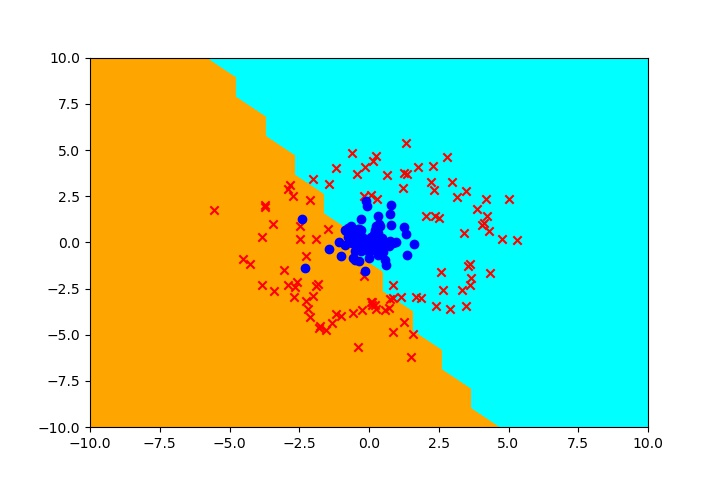
\includegraphics[width=\linewidth]{perceptron_dot_output}
		\caption{Dot-product kernel.}
	\end{subfigure}
	\begin{subfigure}[H]{0.33\linewidth}
		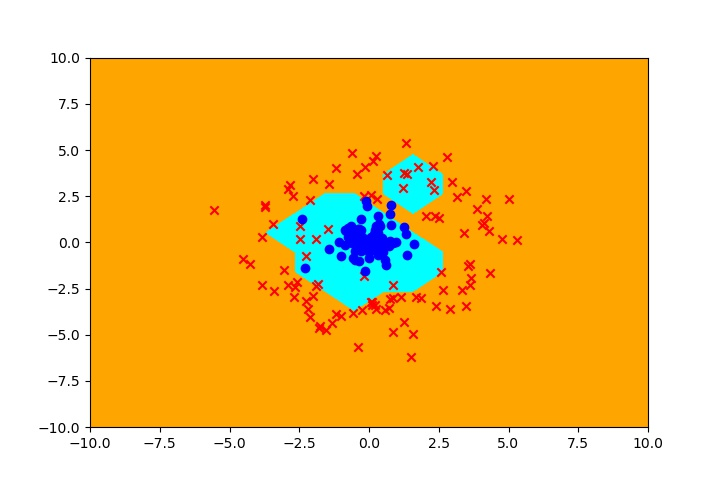
\includegraphics[width=\linewidth]{perceptron_rbf_output}
		\caption{RBF kernel.}
	\end{subfigure}
	\begin{subfigure}[H]{0.33\linewidth}
		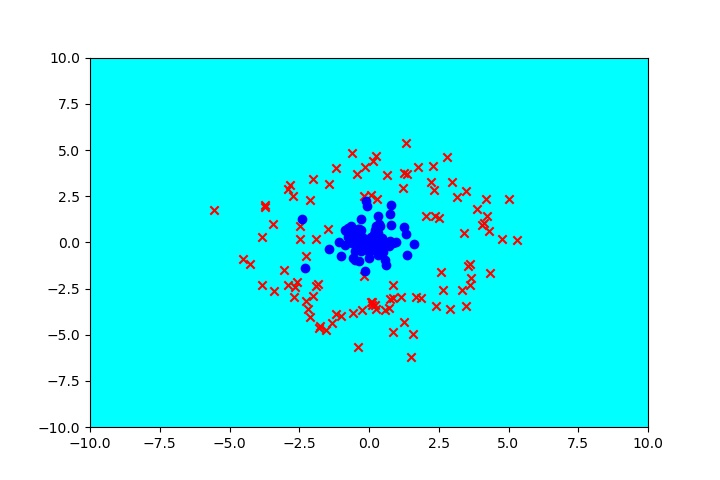
\includegraphics[width=\linewidth]{perceptron_non_psd_output}
		\caption{Not-a-kernel function.}
	\end{subfigure}
	\caption{The Perceptron using different kernels.}
	\end{figure}
\end{answer}

} \fi


  \item \subquestionpoints{2} 
One of the choices in Q4b completely fails, one works a bit, and one works well in classifying the points.
Discuss the performance of different choices and why do they fail or perform well?



\ifnum\solutions=1 {
  \begin{answer}
The dot-product kernel tried to fit a linear decision boundary, this apparently didn't work well on our highly non-linear dataset. Meanwhile, the RBF kernel had an infinite dimensional feature map and was able to learn non-linear decision boundaries (figure 2(b)). Lastly, the not-a-kernel function failed to learn anything useful because it broke the logic of our algorithm. \\
\end{answer}

} \fi

\end{enumerate}
